\documentclass{article}
\usepackage{graphicx}
\usepackage{tabularx}
\usepackage{caption}
\begin{document}
\title{Java Programming Revision Tool}
\author{Nicole Kearns}
\maketitle
\tableofcontents

\newpage

\section{Requirements}

This section discusses the requirements elicitation process for our project. As I have an client, this process is important to ensure that all requirements are identified in order to produce the application that fully meets the clients needs.

\subsection{Student Surveys}

To better my understanding of what would be the most effective tools and features for learning and revising Java programming, I asked a sample of Level 2 and Level 4 students to carry out a survey. The summarised results from both surveys are discussed below.

\subsubsection{Level 4 Student Survey}

In order to gain a better understanding of what students thought of the Java Programming 2 course and to see what features would be beneficial for students learning Java, I spoke to a sample of 10 Level 4 Computing Science students to find out what they thought about the course when they took it 2 years previously. I asked a group of 10 students the following 3 questions:

\begin{enumerate}
\item How useful did you find the material provided for JP2? 
\item What other tools did you use to complete the lab exercises or to learn Java, if any?
\item If you could do the course again, what would you do different? What other tools would you like to be available?
\end{enumerate}

Having recorded the answers from the survey, I have analysed them and have arrived at the following conclusions:\\

From the answers given to question 1 it would seem that, overall, the students thought the material was quite useful, however some improvements could be made. Some students thought that the lecture notes were useful for introducing the basic concepts and syntax of Java. However, when the material became more difficult, the lecture notes lacked detailed information and examples to show how they are used.\\

Most students found that the lab exercises were more beneficial than the lectures as they were able to practice writing Java code, instead of merely reading it. All participants, with one exception, also used extra resources when completing the lab exercises. An example of such is if they came across a problem they were unable to solve. The following resources were the more common ones which were discussed; general internet searching, StackOverflow, and online tutorial videos.\\

When question 3 asked what they would have liked to have been made available, most participants suggested that it would be useful for more examples or snippets of code to be provided within the lectures. This would allow students to understand more fully how the concepts are used in practice. From the feedback given during the survey, consideration could be given to make the lectures more interactive to help the students to stay interested and allow them to practice and improve hand-writing code. Another suggestion was to provide the students with short video tutorials to talk students through more complicated concepts and provide a step-by-step walk-through of how it works and how it its used.\\

Overall, it would seem that the students thought the lectures were adequate, they provided enough information to be useful for exam revision, however they didn't provide enough examples to demonstrate how the concepts are used. From the results collected, I believe that students find interactive tools more useful when learning a programming language as it allows them to practice and improve on writing correct Java code.\\

\subsubsection{Level 2 Student Survey}

To further my understanding of what the second year students think about the current teaching methods of Java within the Java Programming 2 (JP2) course, I asked them to fill out a survey with the following questions:

\begin{enumerate}
\item The material provided for the JP2 course is useful. ( On a scale of strongly agree to strongly disagree)
\item What do you find more useful, the lectures or the lab exercises?
\item What other resources have you used to understand Java concepts and syntax?
\item What resources do you use when you have a specific problem?
\item Is there any other resources you would like to be available within this course to help you learn and revise Java?
\end{enumerate}

\begin{center}
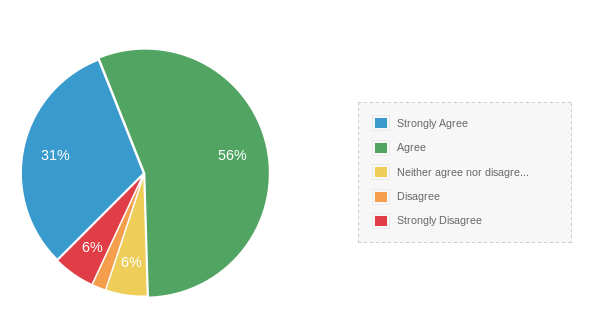
\includegraphics
[scale=0.6]
{/users/level4/0902059k/Level4/Project/L4Project/Dissertation/Requirements/Q1Pie.png}
\end{center}
\begin{center} Question 1 Results \end{center}

From the graph above, you can clearly see that majority of students think that the material provided for the course is very useful, with very few people thinking that it is not.\\

\begin{center}
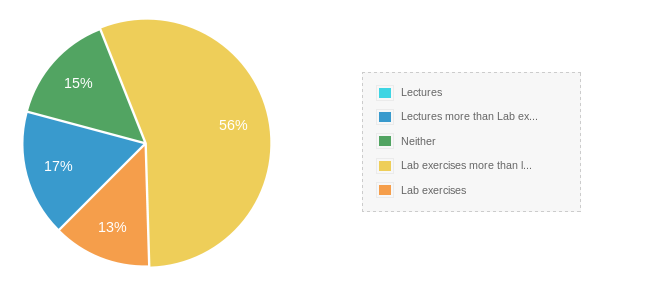
\includegraphics
[scale=0.6]
{/users/level4/0902059k/Level4/Project/L4Project/Dissertation/Requirements/Q2Pie.png}
\end{center}
\begin{center} Question 2 Results \end{center}

For question 2, when asked what they found more useful, lecture notes or lab exercises, it can be said that a vast majority of students find that the lab exercises are more useful, assuming that this is because this allows them to practice writing code.\\

\begin{figure}[!htb]
\minipage{0.6\textwidth}
  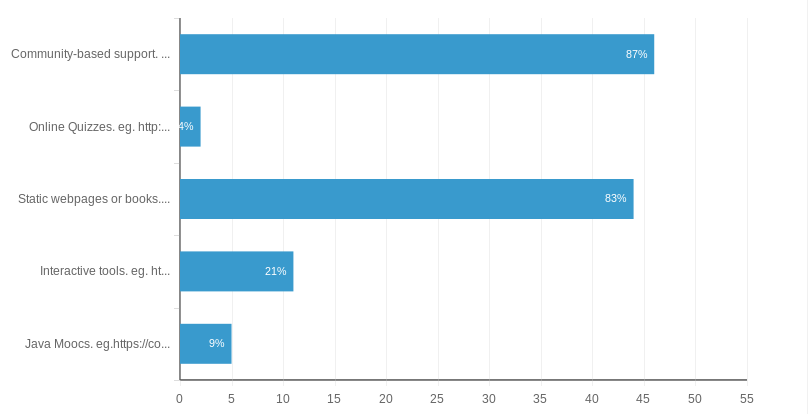
\includegraphics[width=\linewidth]{/users/level4/0902059k/Level4/Project/L4Project/Dissertation/Requirements/Q3Bar.png}
\endminipage\hfill
\minipage{0.6\textwidth}
  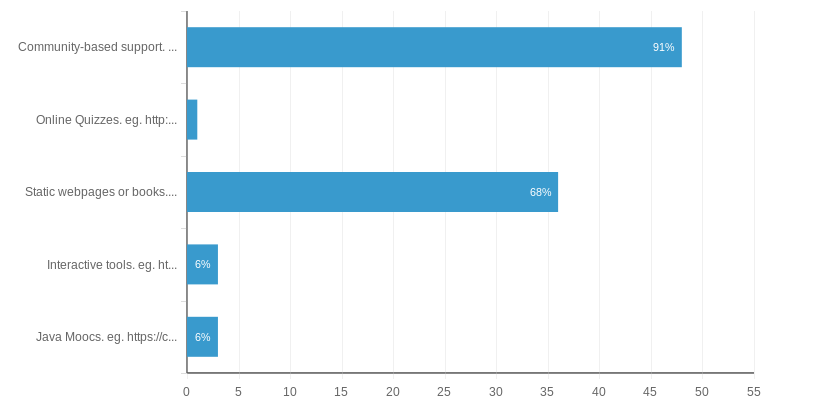
\includegraphics[width=\linewidth]{/users/level4/0902059k/Level4/Project/L4Project/Dissertation/Requirements/Q4Bar.png}
\endminipage\hfill
\end{figure}


For questions 3 and 4, it would seem that students use the same resources for both learning Java and for referring to when they encounter a problem. The resources which are most popular with the students are community-based support and static webpages/books. Community-based support allows the user to ask questions or post problems that they are struggling with, answer questions from other people, and simply view problems and solutions from other users.\\

A few suggestions were given for tools and facilities which they would like to be available are:

\begin{itemize}
\item Video tutorials.
\item Mini exercises to create fun mini projects.
\item The code provided in class to be provided in the notes or on moodle.
\item Plenty of exercises and examples, especially to emphasise OO programming.
\item A more simplified explanation of the basics.
\end{itemize}

\subsection{Functional Requirements}

From the information and suggestions provided by both the Level 2 and Level 4 Computing Science students, I produced the following list of requirements for the application which I think would be most benefitial to the students:

\begin{itemize}
\item Provide the students with multiple activities which will allow them to practice and learn Java.
\item Provide the students with tutorials which go through the basic syntax and Java concepts.
\item Provide video tutorial to allow the students to revise and learn.
\item Allow lecturer/admin to add and update content - questions and quizzes
\end{itemize}

The activities which the client and I thought would be most benefitial to the students for learning and practicing Java code are:\\

\begin{itemize}
\item \textbf{Multiple Choice Questions} in which the user is provided with questions about Java syntax and snippets of code in which they must predict the output. This allows the user to improve their ability to read lines of code and understand it's behaviour.
\item \textbf{Fill in the Blanks Questions} which provide the user with a small sample of code which a Java keyword removed and the user must enter the keyword which will complete the line of code.
\item \textbf{Find the Errors.} This provides students with a piece of code, which contains errors and the user must identify where in the code the errors lie. This will enhance the users ability to read code, predict it behaviour and identify where the errors occur.
\item \textbf{Code your Own}, a section which provides the user with a question or scenario in which the user must write the own code in order to complete the task.
\end{itemize}

\subsubsection{Requirements Table}

\textbf{Student - } Uses the application to learn and revise Java using the activities provided; answering the multiple choice questions, completing the Fill in the Blank questions, identifying the errors within the broken code provided and writing their own code. Also through browsing the tutorials and video tutorials which will go over the basic Java syntax and concepts.\\
\\
\textbf{Lecturer - } Responsible for adding content to the application such as the questions for all relevant activities, the tutorials and video tutorials.\\


\textbf{Student Requirements}\\

\begin{center}
\begin{tabular}{l*{3}{c}r}
\hline
\textbf{Id} & \textbf{Requirement} & \textbf{Description} & \textbf{Priority}\\
\hline
SR1 & \multicolumn{1}{m{4cm}}{View Tutorials} & \multicolumn{1}{m{8cm}}{Responsible for adding content to the application such as the questions for all relevant activities, the tutorials and video tutorials.} & Must Have\\
SR2 & \multicolumn{1}{m{4cm}}{View Video Tutorials} & & Must Have\\
SR3 & \multicolumn{1}{m{4cm}}{View Questions} & & Must Have\\
SR4 & \multicolumn{1}{m{4cm}}{Answer Questions for Multiple Choice and Fill in the Blanks} & & Must Have\\
SR5 & \multicolumn{1}{m{4cm}}{Write Java code and execute it for Code Your Own} & & Must Have \\
SR6 & \multicolumn{1}{m{4cm}}{Edit the provided Java code and execute it for Find the Errors} & & Must Have \\
\hline 
\end{tabular}
\end{center}

\textbf{Lecturer Requirements}\\

\begin{center}
\begin{tabular}{|c|c|c|c|}
\hline \textbf{Id} & \textbf{Requirement} & \textbf{Description} & \textbf{Priority}\\
\hline LR1 & Add Tutorials & & Must Have\\
\hline LR2 & Edit Tutorials & & Should Have\\
\hline LR3 & Delete Tutorials & & Must Have\\
\hline LR4 & Add Video Tutorials & & Must Have\\
\hline LR5 & Edit Video Tutorials & & Should Have\\
\hline LR6 & Delete Video Tutorials & & Must Have\\
\hline LR7 & Add Questions & & Must Have\\
\hline LR8 & Edit Questions & & Should Have\\
\hline LR9 & Delete Questions & & Must Have\\
\hline 
\end{tabular}
\end{center}



\end{document}
